\section{ディレクトリ構成}

\begin{figure}[t]
\begin{center}
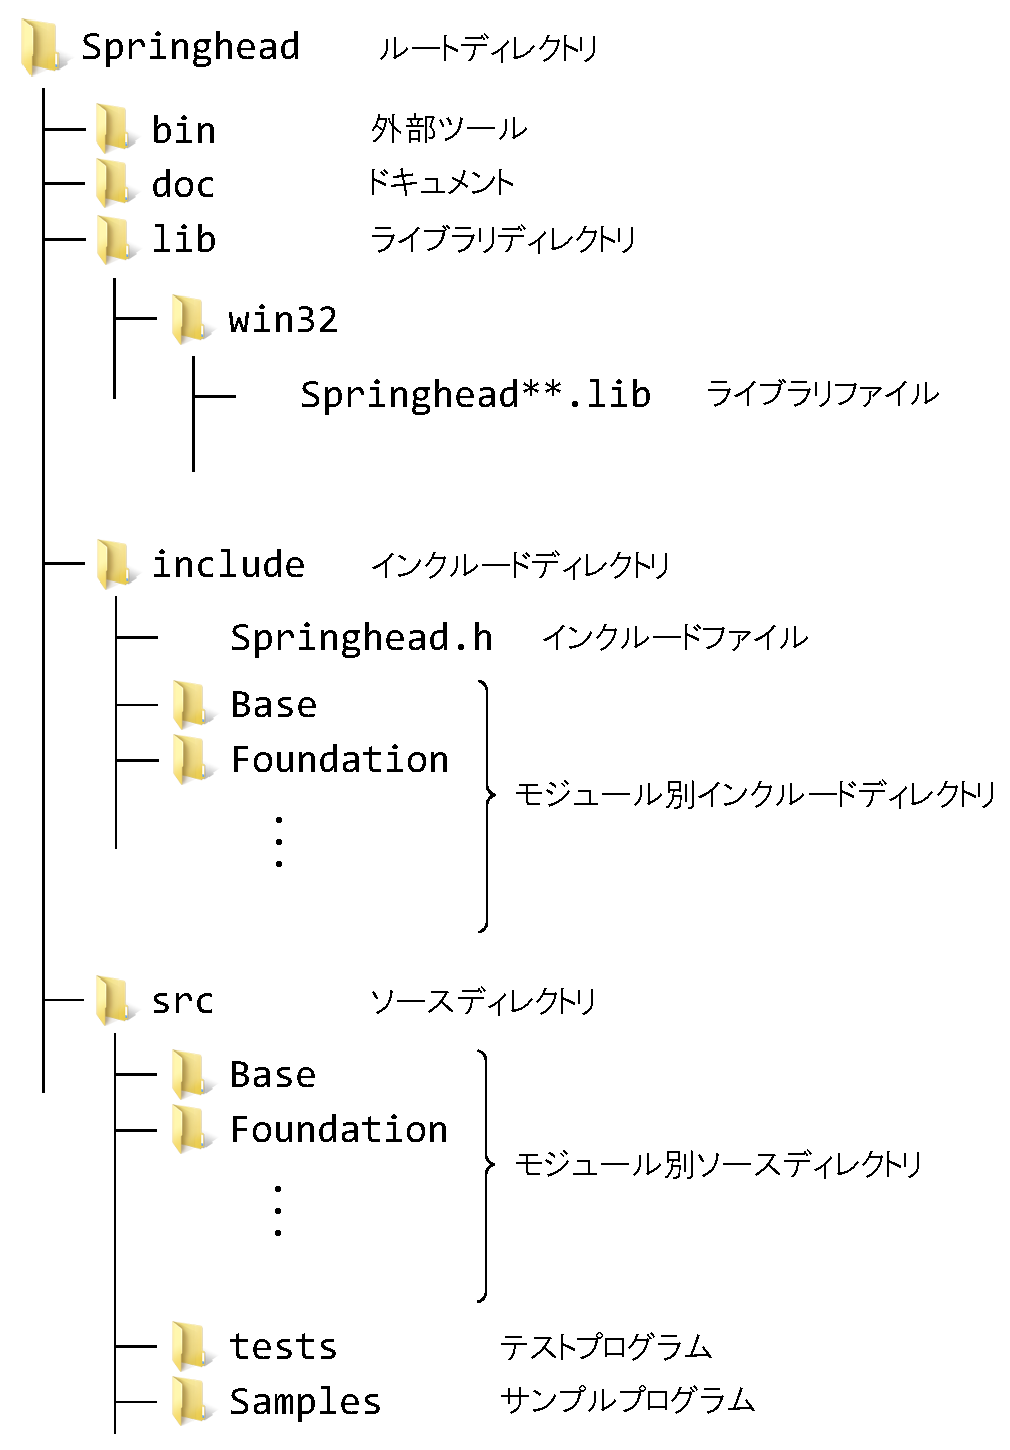
\includegraphics[width=.6\hsize]{fig/filetree.eps}
\end{center}
\caption{Directory tree of Springhead}
\label{fig_filetree}
\end{figure}

Springheadのディレクトリ構成をFig.\,\ref{fig_filetree}に示します.

\section{ライブラリ構成}

\begin{table}[t]
\caption{Springhead modules}
\label{table_modules}
\begin{tabular}{lll}
\toprule
\KLUDGE モジュール名			& プリフィックス	& 機能	\\ \midrule
{\bf Base}				& -					& 行列・ベクトル演算,スマートポインタ,\\
						&					& その他基本機能	\\
{\bf Foundation}		& UT				& Springheadの基本クラス,実行時型情報	\\
{\bf Collision}			& CD				& 衝突判定	\\
{\bf Physics}			& PH				& 物理計算	\\
{\bf Graphics}			& GR				& シーングラフ,描画	\\
{\bf FileIO}			& FI				& ファイル入出力	\\
{\bf HumanInterface}	& HI				& ヒューマンインタフェースデバイスや \\
						&					& インタラクション \\ 
{\bf Creature}			& CR				& バーチャルクリーチャ \\
{\bf Framework}			& FW				& モジュール間の連携と \\
						&					& アプリケーション作成支援 \\ \bottomrule
\end{tabular}
\end{table}

\begin{table}[t]
\caption{Module dependencies}
\label{table_dependency}
\begin{center}
\begin{tabular}{llllllllll}
\toprule
\KLUDGE モジュール名			& 			&			&			&			&			&			&			&			&			\\ \midrule
{\bf Base}				& -			& -			& -			& -			& -			& -			& -			& -			& -			\\
{\bf Foundation}		& $\circ$	& -			& -			& -			& -			& -			& -			& -			& -			\\
{\bf Collision}			& $\circ$	& $\circ$	& -			& -			& -			& -			& -			& -			& -			\\
{\bf Physics}			& $\circ$	& $\circ$	& $\circ$	& -			& -			& -			& -			& -			& -			\\
{\bf Graphics}			& $\circ$	& $\circ$	& -			& -			& -			& -			& -			& -			& -			\\
{\bf FileIO}			& $\circ$	& $\circ$	& -			& -			& -			& -			& -			& -			& -			\\
{\bf HumanInterface}	& $\circ$	& $\circ$	& -			& -			& -			& -			& -			& -			& -			\\
{\bf Creature}			& $\circ$	& $\circ$	& -			& $\circ$	& -			& -			& -			& -			& -			\\
{\bf Framework}			& $\circ$	& $\circ$	& -			& $\circ$	& $\circ$	& $\circ$	& $\circ$	& -			& -			\\ \bottomrule
\end{tabular}
\end{center}
\end{table}

Springheadは複数のモジュールから構成されています.
Table\,\ref{table_modules}にモジュール一覧を示します.
Table\,\ref{table_dependency}にモジュール間の依存関係を示します.
\KLUDGE 通常,ユーザはSpringheadを使用するにあたってこれらの依存関係を陽に意識する必要はありません.
\KLUDGE また,何らかの事情でSpringheadの特定の機能(たとえば物理シミュレーション)のみを用いたいという場合に対応できるように,
\KLUDGE モジュール間の依存関係はなるべく疎になるように設計されています.
\KLUDGE したがってこのような場合には用途に応じて必要なモジュールのみを使えるようになっています.

\section{クラス・APIの命名規則}

\KLUDGE 各モジュールに含まれるクラスの名前には,Table\,\ref{table_modules}に示されるようなモジュール固有のプリフィックスがつきます
(例: Physicsモジュールの\texttt{PHSolid},Collisionモジュールの\texttt{CDShape}).
\KLUDGE 一部にはこのルールにしたがわないクラスも存在します(例: FoundationモジュールのObject).

API(クラスのメンバ関数)にも緩い命名規則があります.
API名は基本的に(動詞 + 目的語)という形式で処理内容を端的に表現します.
\KLUDGE また,単語の先頭文字のみ大文字,その他は小文字で表記します.
\KLUDGE 例としては\texttt{PHSolid::SetMass},\texttt{GRSdk::CreateScene}などです.

\section{インタフェースとディスクリプタ} 
\label{sec_if_desc}

Springheadでは仕様と実装を明確に分離するために,インタフェースクラスと実装クラスが分けられています.
\KLUDGE ユーザはインタフェースクラスのみを使用してSpringheadの機能を利用します.
\KLUDGE ただし,\url{Base}と\url{Foundation}モジュールにあるごく基本的なクラス,および\url{Framework}のアプリケーションクラスは例外となっています.

\KLUDGE また,Springheadのクラスにはそれぞれにディスクリプタが用意されています.ディスクリプタとは,そのクラスの読み書き可能な属性のみを集めた構造体です.
\KLUDGE ディスクリプタを利用することで,同じ設定のインスタンスを多数設定することが用意になります.
\KLUDGE また,ディスクリプタはファイルへのデータの保存や読み込みにおいても役立ちます.

\KLUDGE 以下に\url{Physics}モジュールの剛体を表す\url{PHSolid}クラスを例にとって説明します.
\begin{sourcecode}
// given PHSolidIf* phScene, 

PHSolidDesc desc;
desc.mass = 1.0;

PHSolidIf* solid = phScene->CreateSolid(desc);
\end{sourcecode}
\KLUDGE 上のコードで\url{PHSolidDesc}は\url{PHSolid}クラスのディスクリプタです.
\KLUDGE まずそのメンバ変数\url{mass}に値をセットすることで剛体の質量を設定しています.
\KLUDGE 次に,剛体を作成するために\url{CreateSolid}関数が呼ばれます.
\KLUDGE ここで\url{CreateSolid}は物理シーンを表す\url{PHScene}クラスのメンバ関数です.
\KLUDGE 実際には\url{PHScene}クラスのインタフェース\url{PHSceneIf}を取得する必要がありますが,ここでは既に得られているとしています.
\KLUDGE 剛体が作成されると,\url{CreateSolid}からインタフェース\url{PHSolidIf}のポインタが返されます.
\KLUDGE これ以降の剛体の操作はこのインタフェースを介して行います.
\begin{sourcecode}
solid->SetMass(5.0);
\end{sourcecode}
\KLUDGE 基本的に,ディスリプタを介して設定可能な属性はインタフェースの\url{Get/Set}系関数を使って取得,設定ができるようになっています.
\KLUDGE 場合に応じて便利な方を使ってください.

Springheadオブジェクトはすべて内部でメモリ管理されていますので,ユーザが明示的に\url{delete}する必要はありません(また,してはいけません).
\url{Create}されたオブジェクトはプログラムの終了時に自動的に破棄されます.

\section*{より詳しく知りたい人は}

\KLUDGE 以降の章では各モジュールについてより詳しく説明します.
Springheadを利用する上で,すべてのモジュールを詳しく理解する必要はありません.
\KLUDGE 必要に応じて参照してください.
